%%%%%%%%%%%%%%%%%%%%%%%%%%%%%%%%%%%%%%%%%
% Stylish Article
% LaTeX Template
% Version 2.1 (1/10/15)
%
% This template has been downloaded from:
% http://www.LaTeXTemplates.com
%
% Original author:
% Mathias Legrand (legrand.mathias@gmail.com) 
% With extensive modifications by:
% Vel (vel@latextemplates.com)
%
% License:
% CC BY-NC-SA 3.0 (http://creativecommons.org/licenses/by-nc-sa/3.0/)
%
%%%%%%%%%%%%%%%%%%%%%%%%%%%%%%%%%%%%%%%%%

%----------------------------------------------------------------------------------------
%	PACKAGES AND OTHER DOCUMENT CONFIGURATIONS
%----------------------------------------------------------------------------------------

\documentclass[fleqn,10pt]{SelfArx} % Document font size and equations flushed left

\usepackage[english]{babel} % Specify a different language here - english by default

\usepackage{lipsum} % Required to insert dummy text. To be removed otherwise

%----------------------------------------------------------------------------------------
%	COLUMNS
%----------------------------------------------------------------------------------------

\setlength{\columnsep}{0.55cm} % Distance between the two columns of text
\setlength{\fboxrule}{0.75pt} % Width of the border around the abstract

%----------------------------------------------------------------------------------------
%	COLORS
%----------------------------------------------------------------------------------------

\definecolor{color1}{RGB}{0,0,90} % Color of the article title and sections
\definecolor{color2}{RGB}{0,20,20} % Color of the boxes behind the abstract and headings

%----------------------------------------------------------------------------------------
%	HYPERLINKS
%----------------------------------------------------------------------------------------

\usepackage{hyperref} % Required for hyperlinks
\hypersetup{hidelinks,colorlinks,breaklinks=true,urlcolor=color2,citecolor=color1,linkcolor=color1,bookmarksopen=false,pdftitle={Title},pdfauthor={Author}}

%----------------------------------------------------------------------------------------
%	ARTICLE INFORMATION
%----------------------------------------------------------------------------------------

\JournalInfo{CSCI-B565 Data Mining, Spring 2023} % Journal information
\Archive{} % Additional notes (e.g. copyright, DOI, review/research article)

\PaperTitle{Semester Project - Walmart Sales Forecasting} % Article title

\Authors{Shalini Kothuru,
Shivani Chennoju,
NagaJahnavi Dhulipalla,
Venkata Sai Abhigna Devarasetty} % Authors
\affiliation{\textsuperscript{1}\textit{Luddy School of Informatics, Computing, and Engineering, Indiana University, Bloomington, IN, USA}} % Author affiliation


\Keywords{NA as of this phase} % Keywords - if you don't want any simply remove all the text between the curly brackets
\newcommand{\keywordname}{Keywords} % Defines the keywords heading name

%----------------------------------------------------------------------------------------
%	ABSTRACT
%----------------------------------------------------------------------------------------

\Abstract{This project's purpose is to anticipate future sales for Walmart, one of the country's largest retail companies. Accurate sales forecasting is essential for optimizing inventory levels, controlling workforce requirements, and boosting customer satisfaction. We want to address the intricacies of Walmart's business strategy, which can be influenced by a range of factors including seasonal trends, promotions, and regional market circumstances. We found and evaluated many cutting-edge solutions to this challenge, including time series and ensemble approaches. We hope to contribute to Walmart's operational success, improve its financial performance, and apply and extend our skills in data mining, machine learning, and other important sectors by enhancing the accuracy of its sales projections.}

%----------------------------------------------------------------------------------------

\begin{document}

\flushbottom % Makes all text pages the same height

\maketitle % Print the title and abstract box

\tableofcontents % Print the contents section

\thispagestyle{empty} % Removes page numbering from the first page




%----------------------------------------------------------------------------------------
%Problem and Data Description
%----------------------------------------------------------------------------------------


\section{Problem and Data Description} % The \section*{} command stops section numbering
\subsection{Problem}
The goal of our project is to forecast future sales for Walmart. Walmart is a retail chain, with
many stores across the United States, and accurately forecasting sales is critical for optimizing
inventory levels, managing staffing needs, and solving other business-related problems. The complexity of the Walmart business model is one of the major difficulties in solving this data mining
problem. Sales can be affected by a variety of variables, such as seasonal trends, promotions,
and regional market circumstances. The accuracy of the forecast may also be impacted by errors
or inconsistencies in the data used for this project. Addressing these limitations would be an
important aspect of our project.

\subsection{Data Description}
We are using four datasets for our project: ' calendar', 'sell\_prices', 'sales\_train validation', and 'sales\_train\_evaluation'.

\item \textbf{1. Calendar dataset:}
It includes information on the dates on which the products are sold
\item \textbf{Attributes Information of Calendar:}
\item Date: Calendar Date
\item wm\_yr\_wk: Walmart internal week count(unique for a week)
\item weekday: represents days of the week (Starting from Saturday as 1 and ending with Friday as 7)
\item month, year: represent the current year and month of the calendar
\item d: Can be indexed, which helps in individually identifying the records
\item event\_name\_1, event\_type\_1, event\_name\_2, event\_type\_2: Represent if there is any festival/holiday and their type
\item snap\_CA, snap\_TX, snap\_WI: This tells us whether it is a SNAP day or not (Supplemental Nutrition Assistance Program)

\item \textbf{2. sell\_prices:}
\item It includes data on the prices of products sold per store and the day they were sold.
\item \textbf{Attributes Information of sell\_prices:}
\item store\_id: an identifier for a store where the product is sold
\item item\_id: an identifier for a product
\item wm\_year\_week: a string representing the sale's year and week. (e.g. "2011-01" represents the first week of 2011)
\item sell\_price: the cost of the product during that week.


\item \textbf{3. sales\_train validation:}
\item It includes daily unit sales statistics for each product and retailer from d\_1 to d\_1913
\item \textbf{Attributes Information of sales\_train validation:}

\item id: a unique identifier.
\item item\_id: an identifier for a product
\item dept\_id: an identifier for a department 
\item cat\_id: an identifier for a category 
\item store\_id: an identifier for a store where the product is sold.
\item d\_1 to d\_1913: is an identifier for a product sold each day.

\item \textbf{4. sales\_train\_evaluation:}
\item It has similar data to sales\_train validation but this dataset is used to validate the model.

\bigskip
\bigskip

%----------------------------------------------------------------------------------------
%	Data Preprocessing $\&$ Exploratory Data Analysis
%----------------------------------------------------------------------------------------

\section{Data Preprocessing $\&$ Exploratory Data Analysis} % The \section*{} command stops section numbering


\subsection{Handling Missing Values}
We found that none of the datasets contains null values or missing information except the calendar dataset. These columns have values only when there is an event on that particular day whereas, for other days, it has NaN values. We have replaced these NaN with 'No event'.
\subsection{Exploratory Data Analysis}
As we explored the data, we have derived the following insights from the given datasets. However, we don't have any scope to normalize or scale the data as it is already in a normalized state. Also, all the features are important. So we will be including all the features for the model building in the next phase.
\item \textbf{1. Calendar dataset:}
\item We have nearly 5.5 years of data from 29th January 2011 to 19th June 2016
\item We have 30 unique events from event\_name\_1 and 4 from event\_name\_2
\item On average, we have 5.5 holidays per year (avg holidays = total holidays/total time period = 30/5.5 i.e nearly 5.5 holidays). This indicates that we might have at least 5 upward trends in sales.
\includegraphics[scale=0.5]{}

\item \textbf{2. sell\_prices:}
\item This dataset includes sales information of items sold in 4 different stores in California ('CA\_1', 'CA\_2', 'CA\_3', 'CA\_4') and 3 different stores in Texas('TX\_1', 'TX\_2', 'TX\_3') and 3 different stores in Wisconsin('WI\_1', 'WI\_2', 'WI\_3'). In total 10 different stores.
\item There are three different categories foods, household, and hobbies, and there is more number of items for sale from the foods category followed by household and hobbies.
\item By understanding the data, it is found that the item having the highest average sale price is HOUSEHOLD\_1\_060, with an average sale price being 29.94.
\item After finding the items with the highest average sell price per store, it can be seen that the items related to hobbies are expensive in stores in California('CA\_1', 'CA\_2', 'CA\_3' and 'CA\_4') and also in Washington('WI\_1', 'WI\_2' and WI\_3) and items related to the household are expensive in stores of Texas('TX\_1', 'TX\_2', 'TX\_3').
\item It can be seen that there are many price variations in the items belonging to foods and households, but there is less price variation for items related to hobbies.

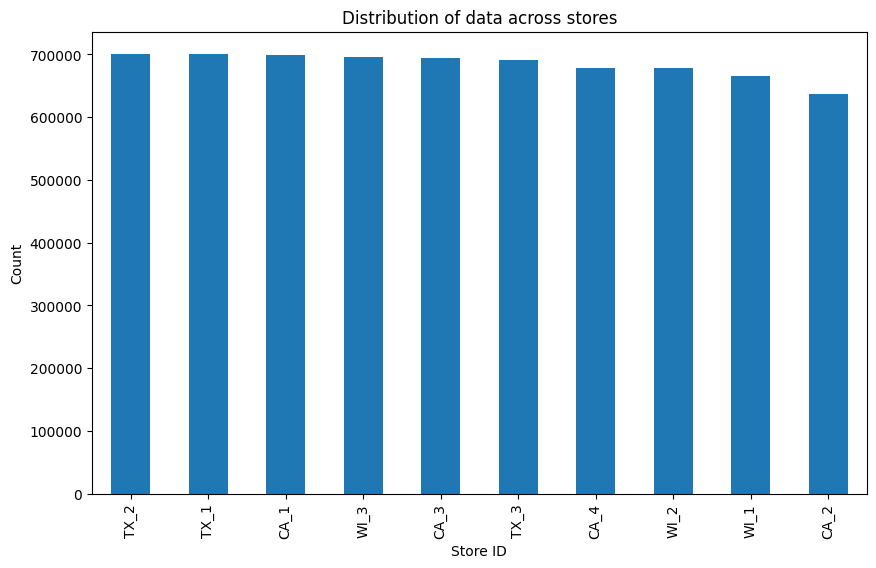
\includegraphics[scale=0.4]{21.png}

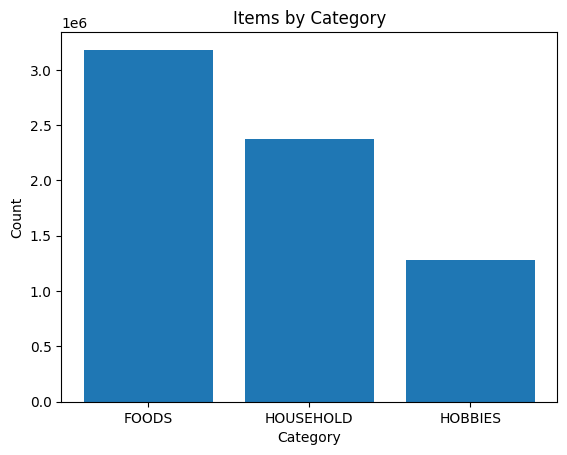
\includegraphics[scale=0.5]{22.png}

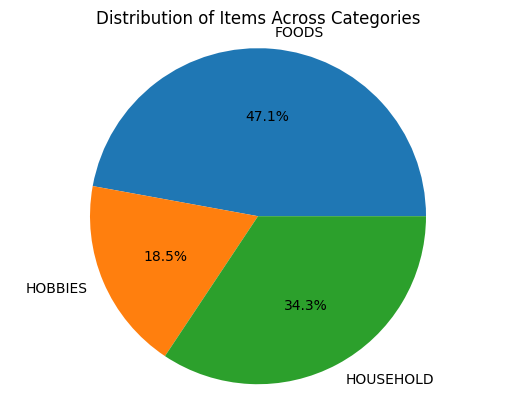
\includegraphics[scale=0.5]{23.png}

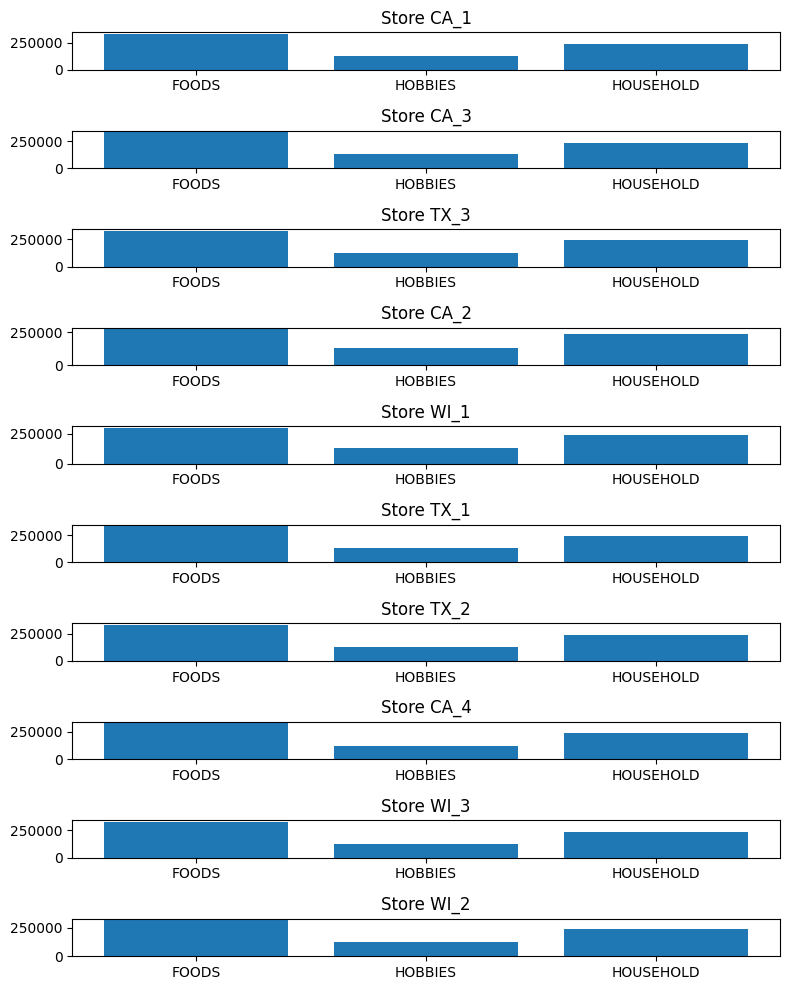
\includegraphics[scale=0.4]{24.png}

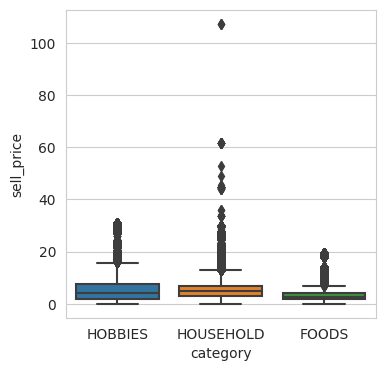
\includegraphics[scale=0.7]{25.png}

\item \textbf{3. sales\_train validation:}

\item We have more sales in California when compared to Texas and Wisconsin.
\item There are three different categories foods, household and hobbies, and there are more number of items for sale from foods category followed by household and hobbies.
\item When compared with the different stores in different states, the sales in CA\_3 have the most sales.
\item In California the sales during the starting period were around 10,000 and then gradually at the end of the period they increased to approx 25,000. Texas and Wisconsin sales are almost the same at the end of the period but at the starting point, Texas has more sales compared to Wisconsin.
\item In California state the highest sales occurred in the CA\_3 store and the lowest was in the CA\_4 store.
\item In Texas state, all stores have the approx same sales towards at end of the period. While at the starting the TX\_2 store has the highest sales.
\item In Wisconsin, the store WI\_3 has the highest sales at the start but it gradually decreased at the end of the period whereas it is quite opposite in the sales of the store WI\_2.

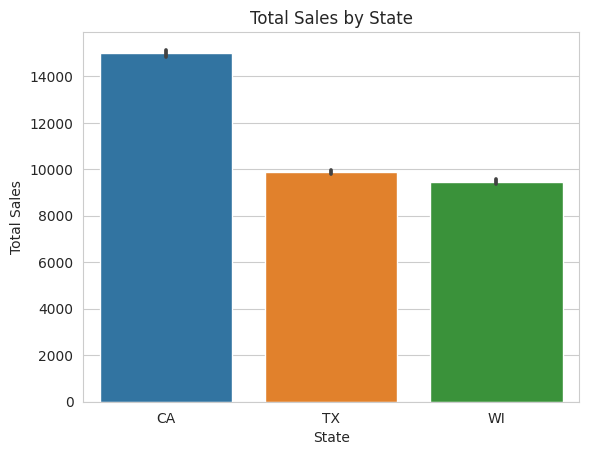
\includegraphics[scale=0.5]{31.png}

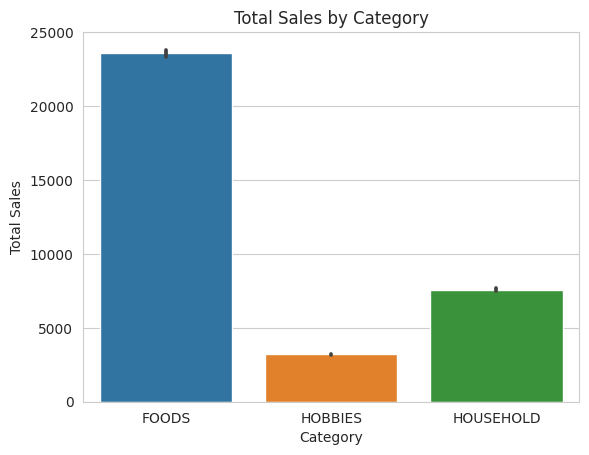
\includegraphics[scale=0.5]{32.png}

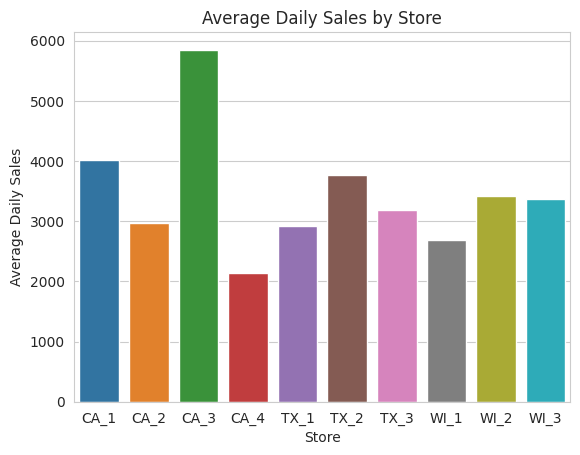
\includegraphics[scale=0.5]{33.png}

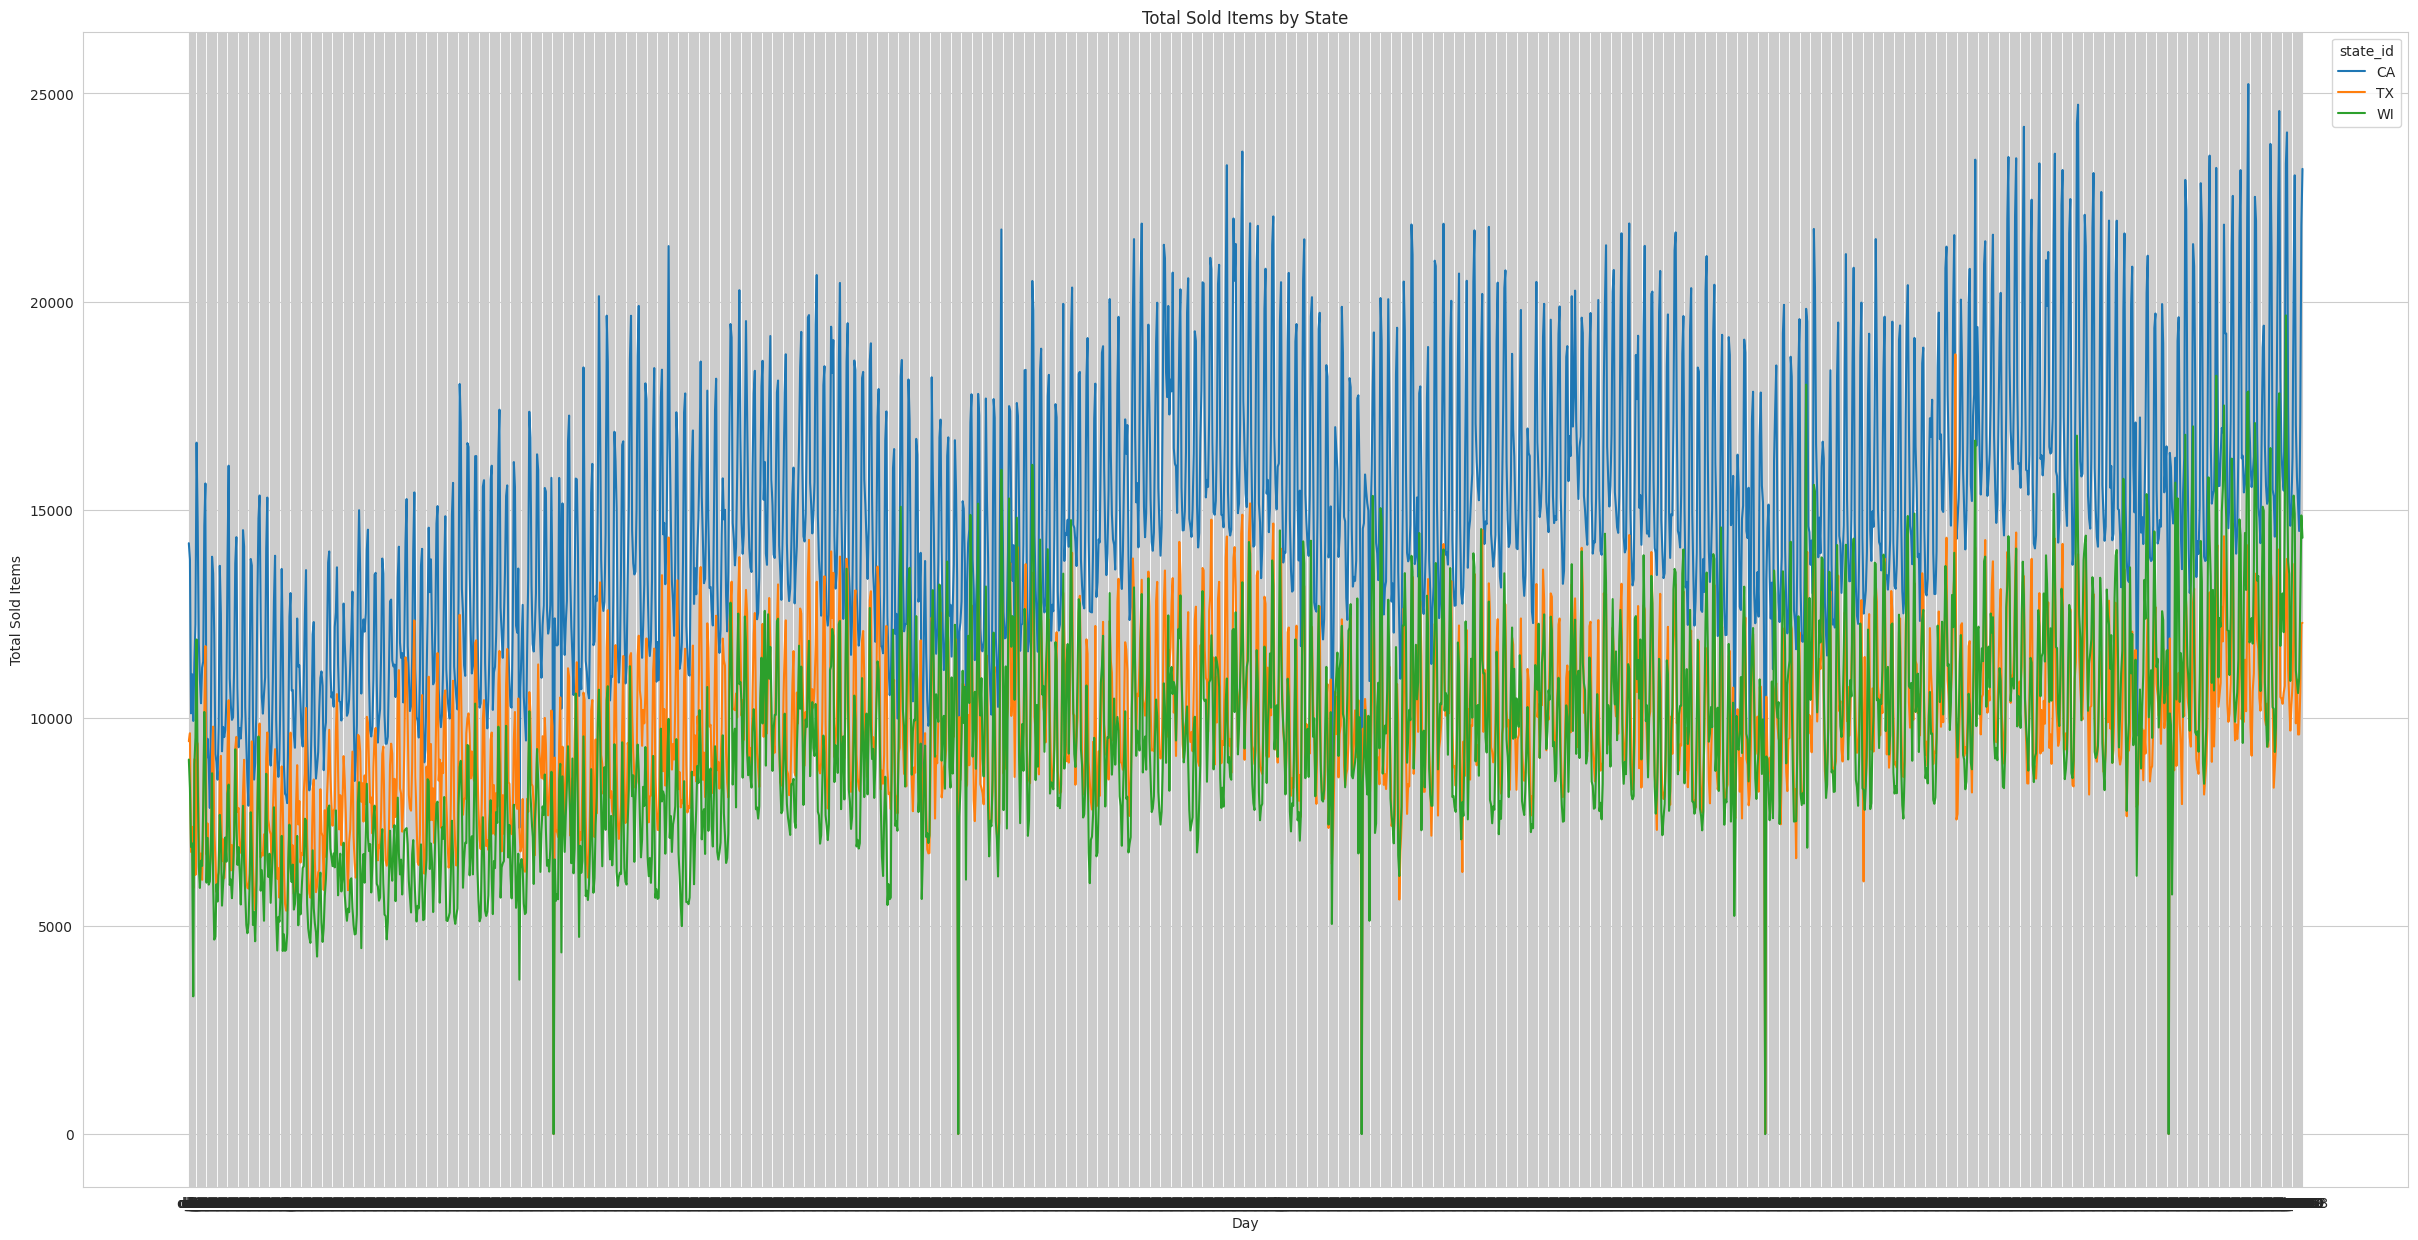
\includegraphics[scale=0.1]{34.png}

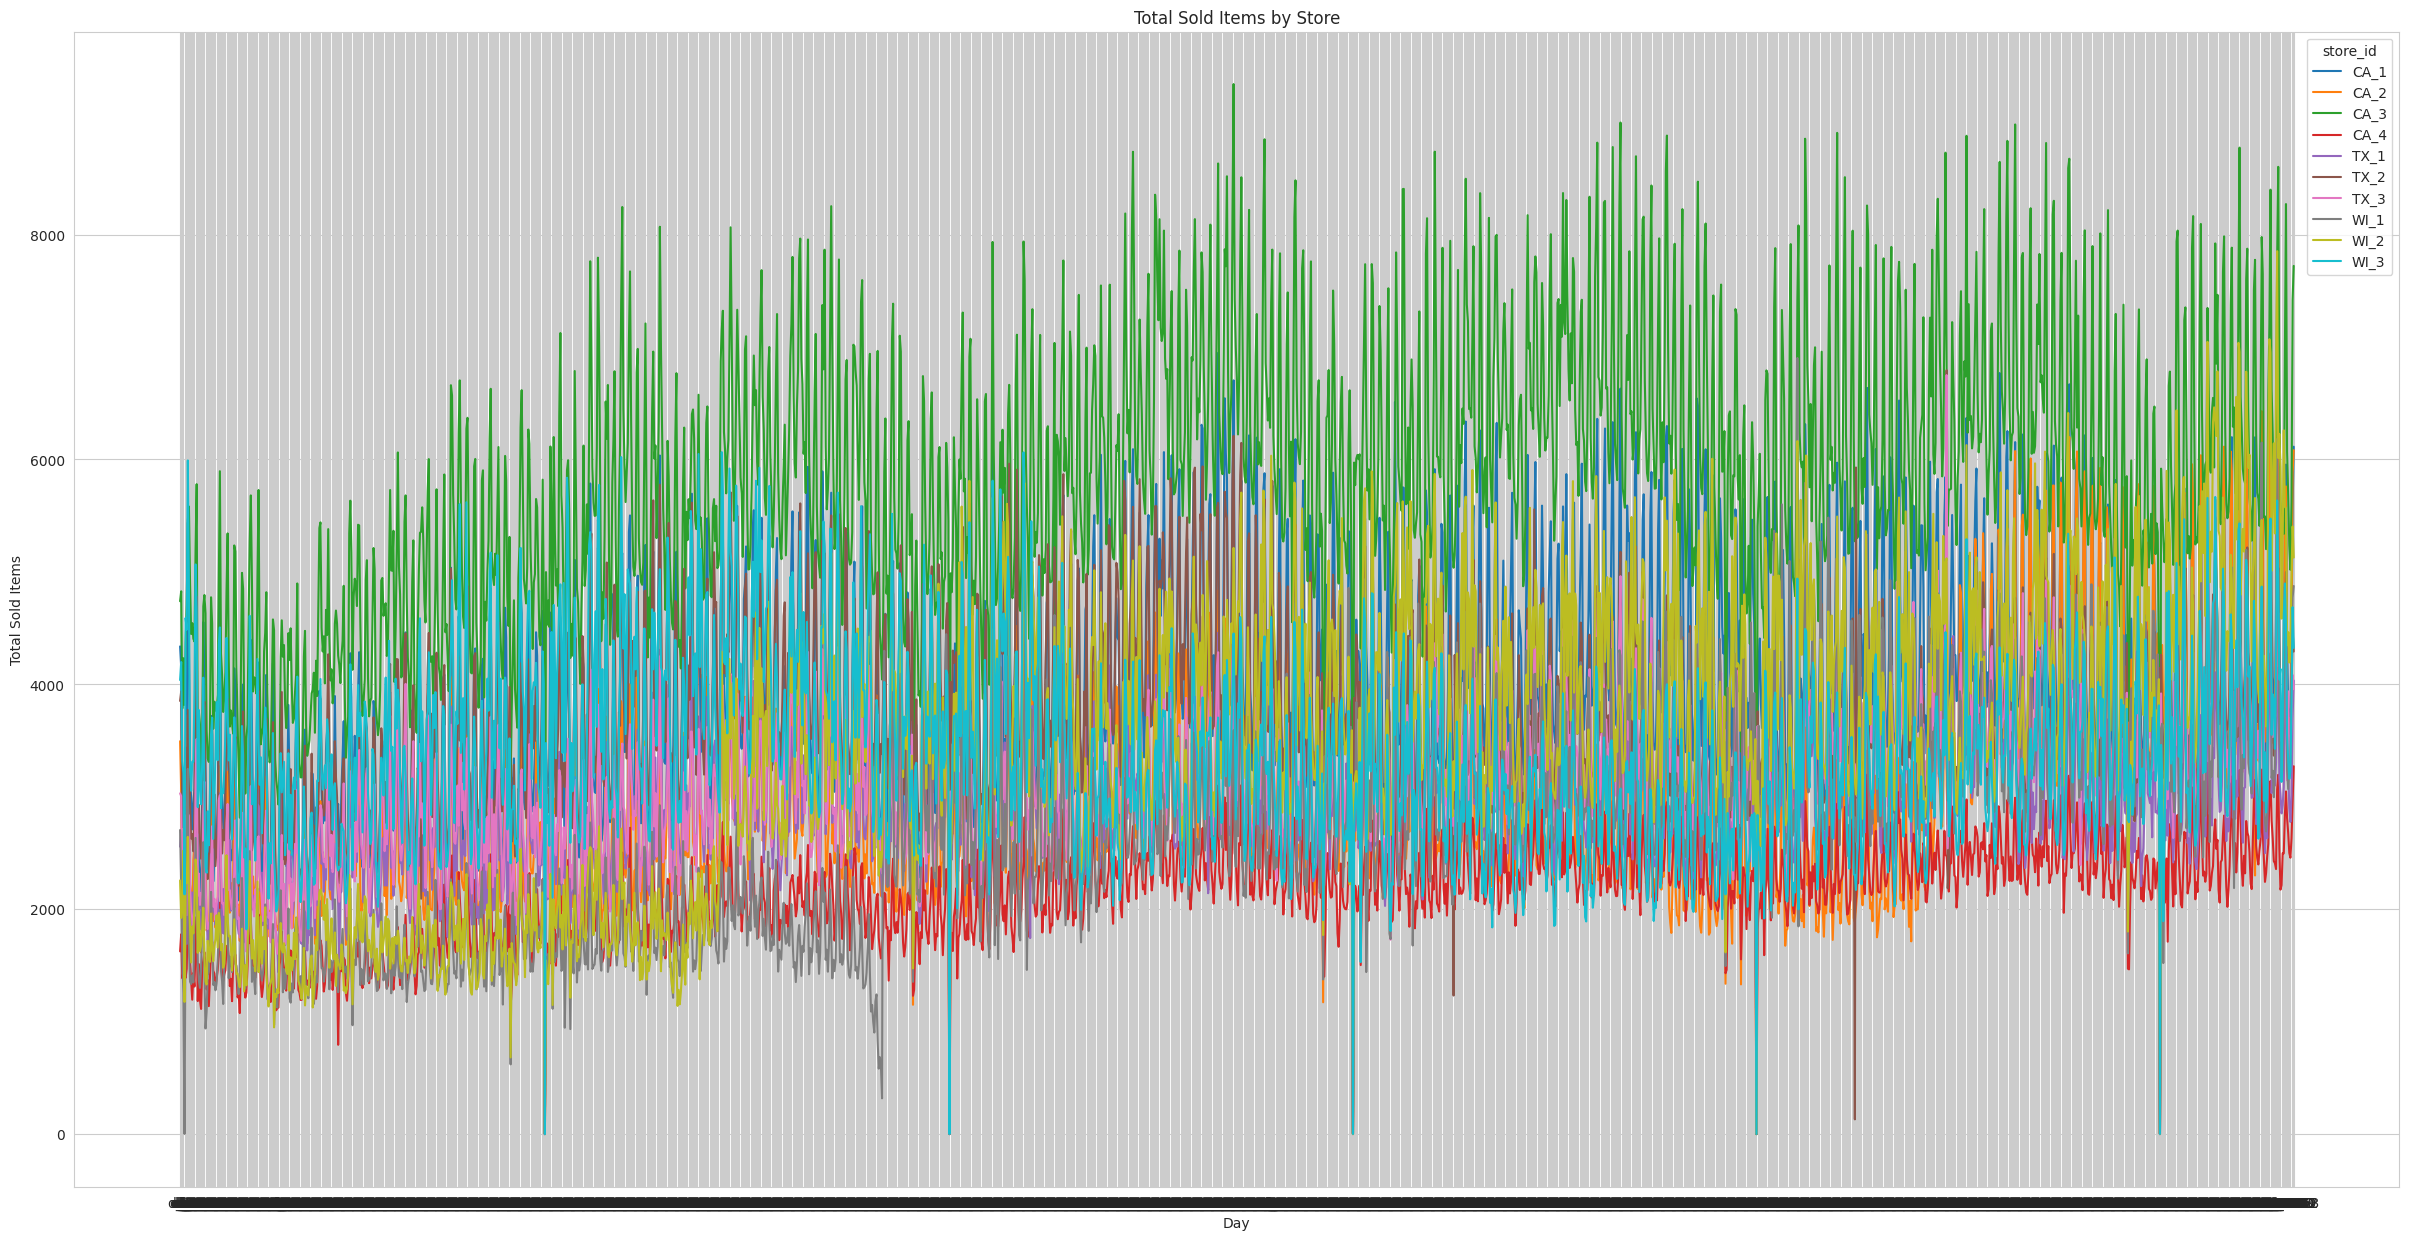
\includegraphics[scale=0.1]{35.png}

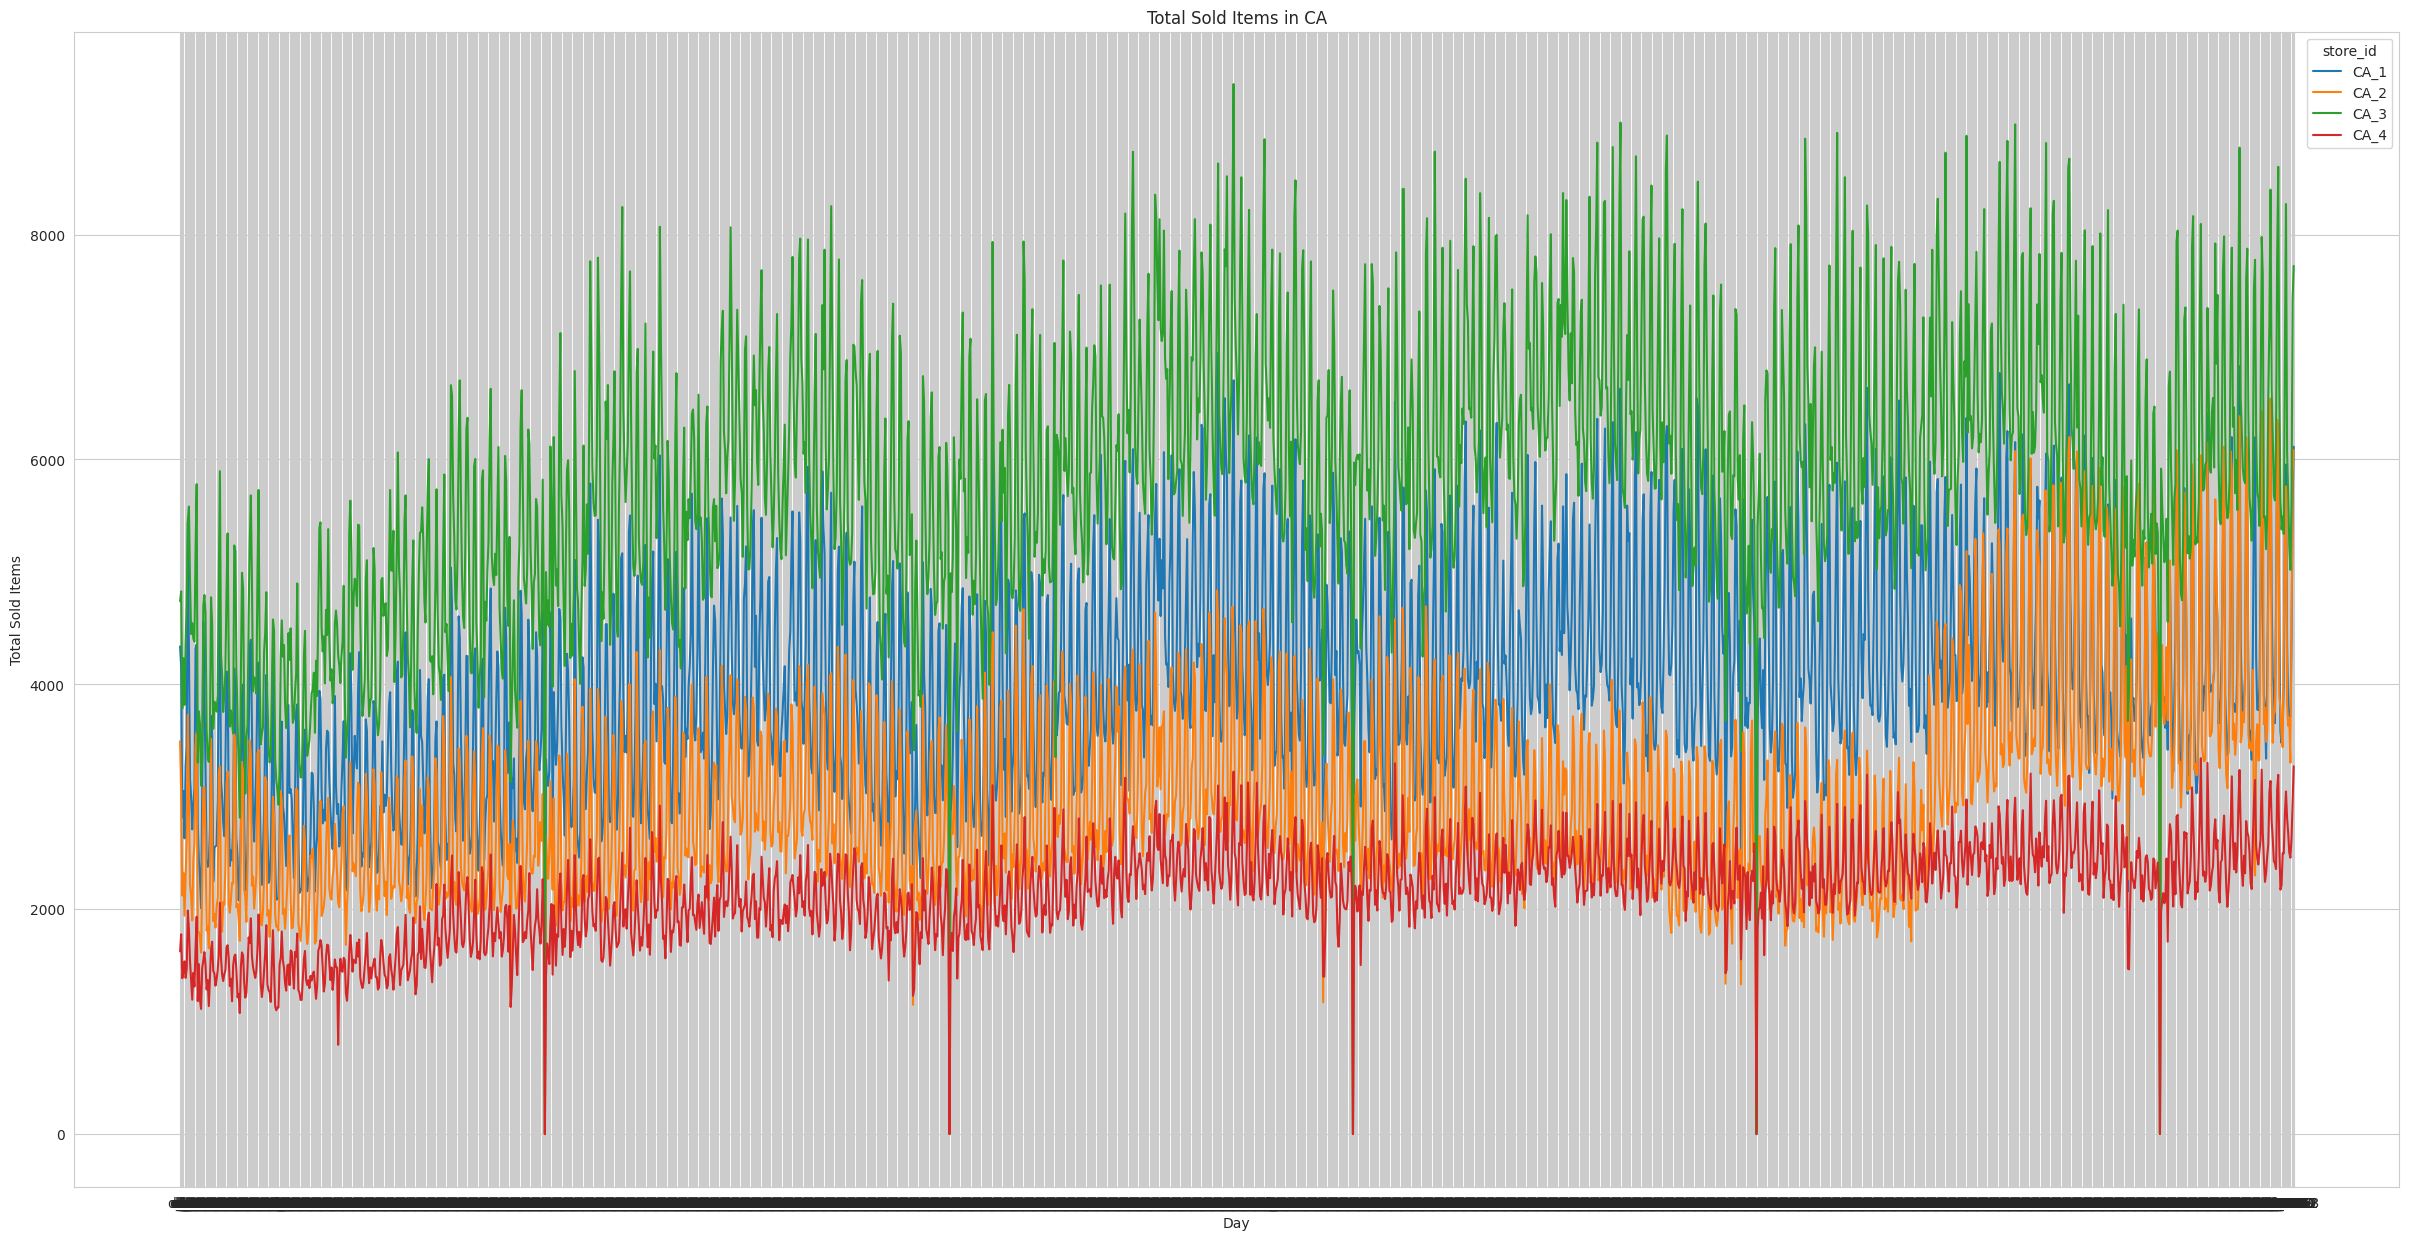
\includegraphics[scale=0.1]{36.png}

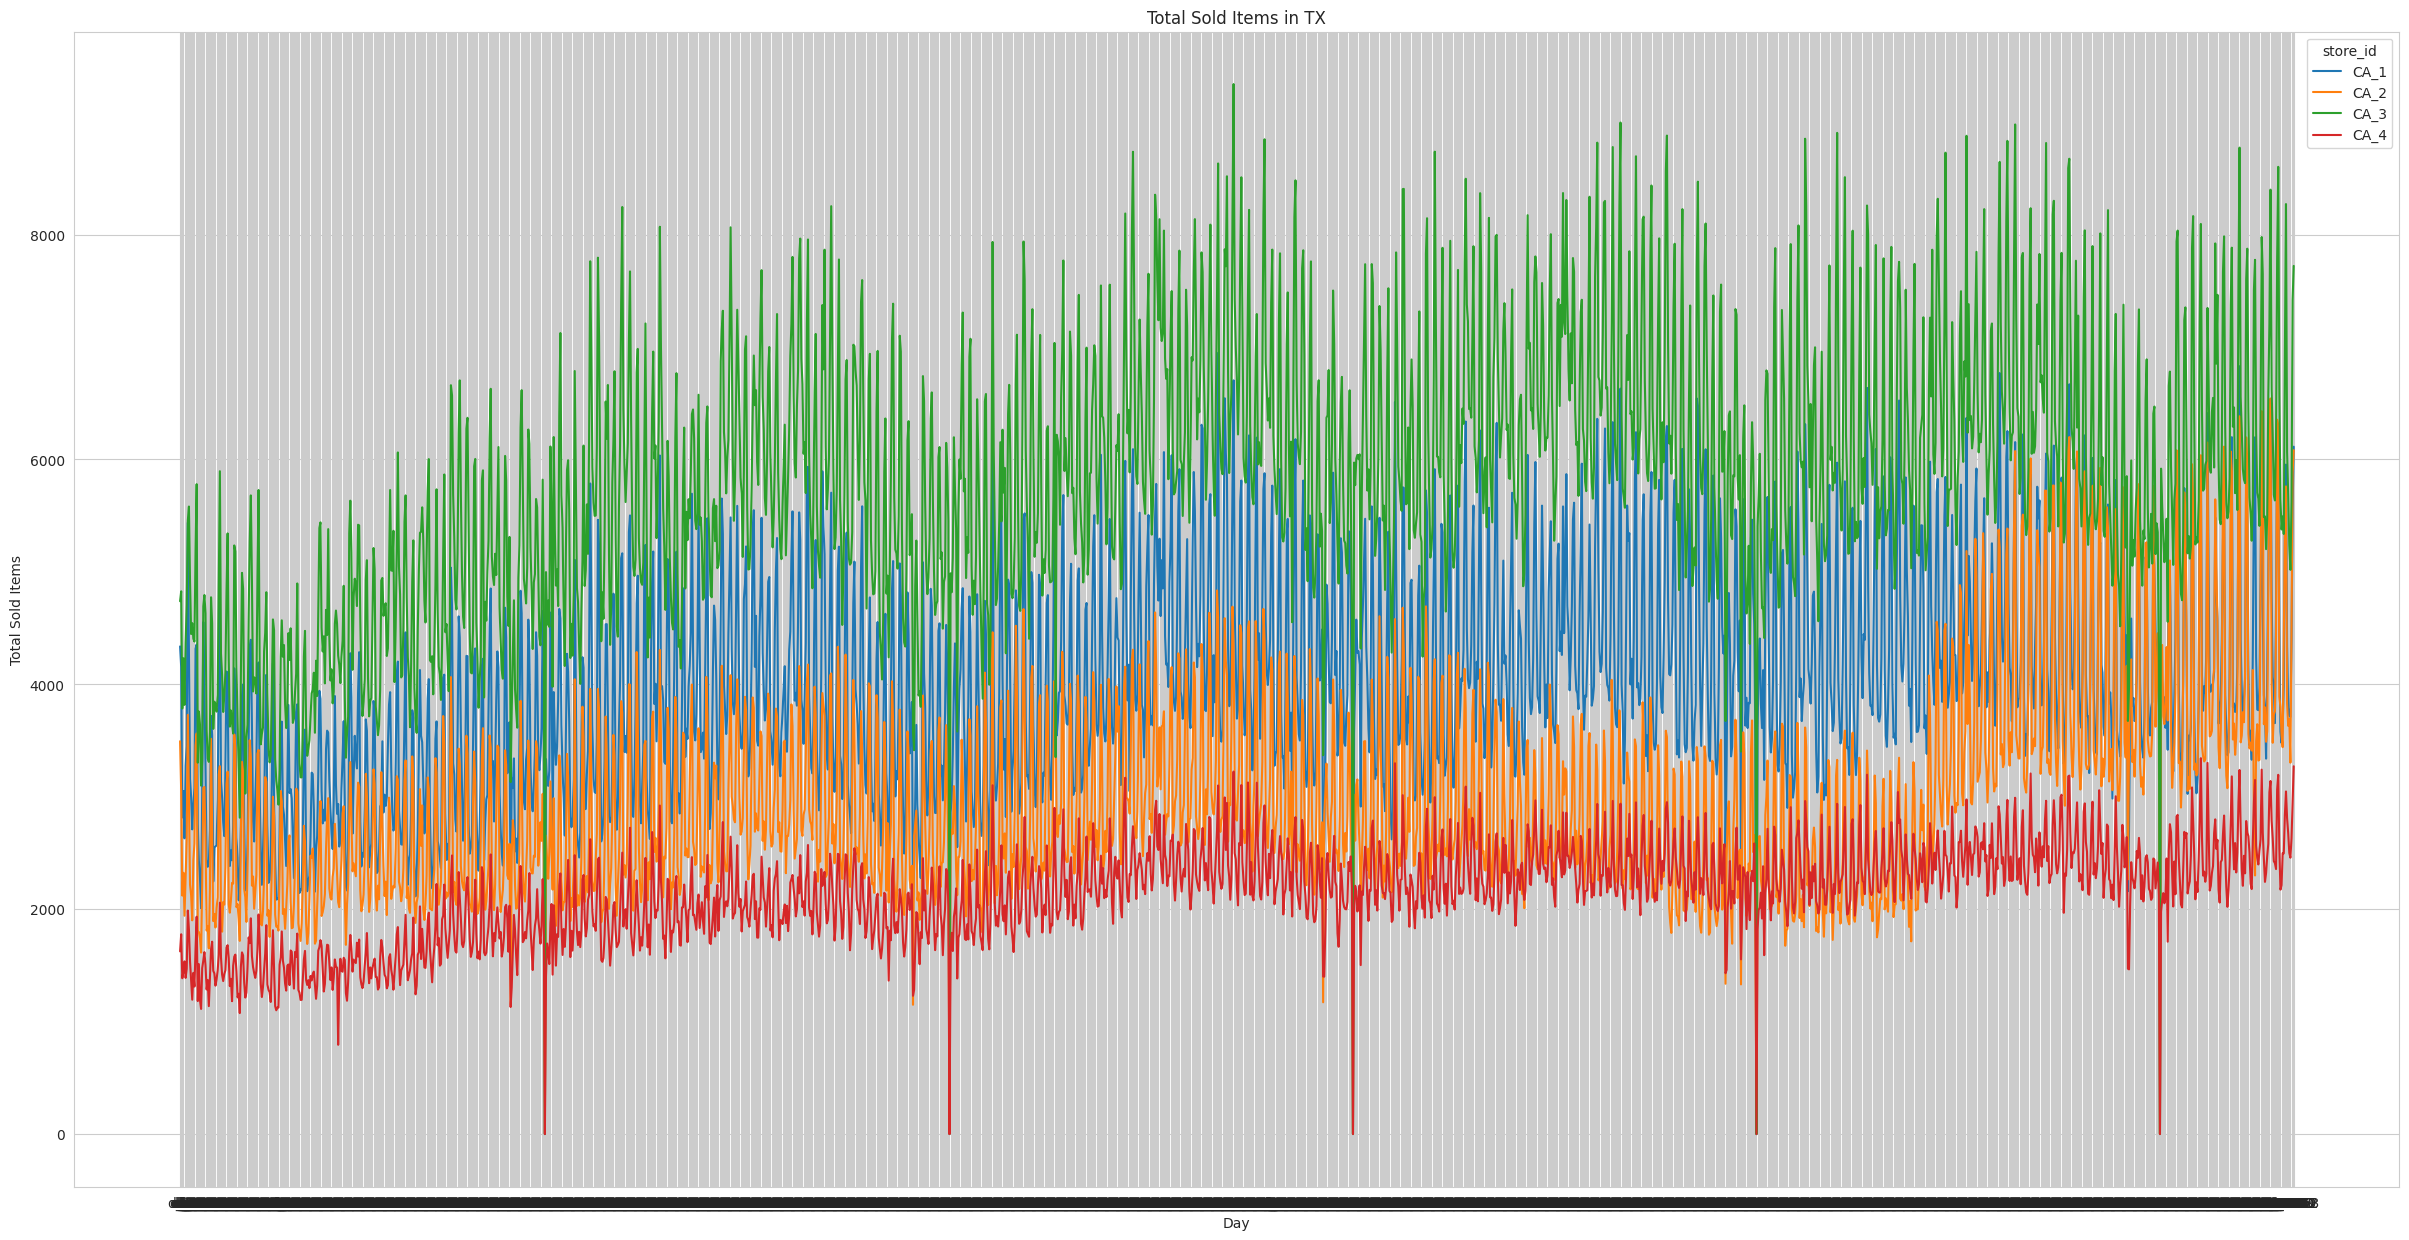
\includegraphics[scale=0.1]{37.png}

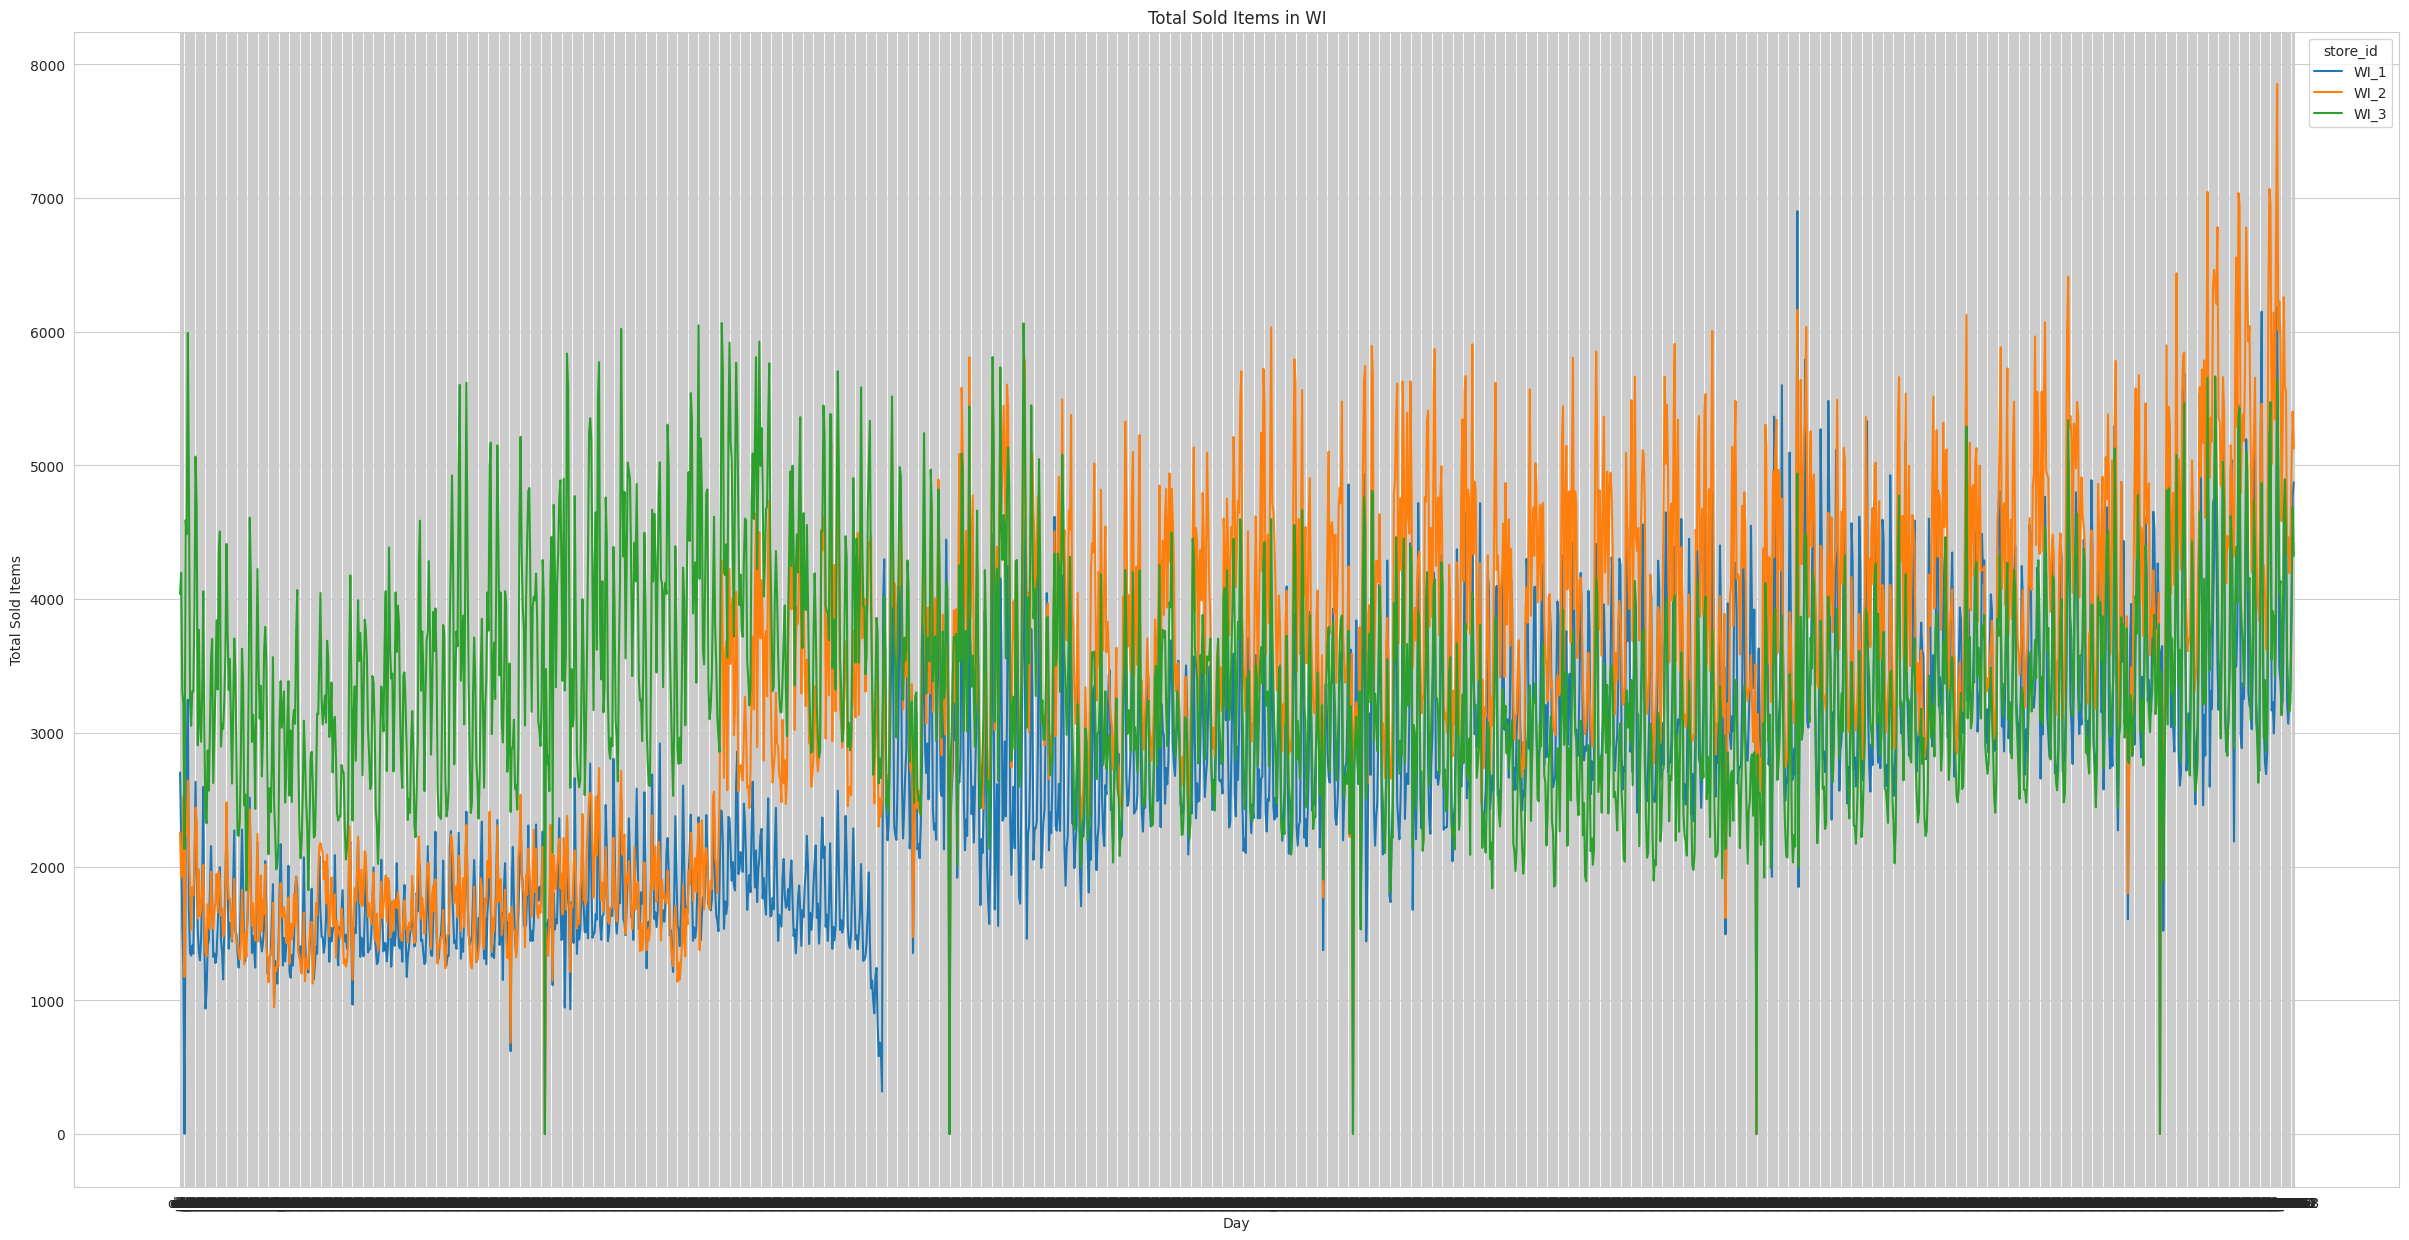
\includegraphics[scale=0.1]{38.png}

\item \textbf{4. sales\_train\_evaluation:}
This dataset will be used for validation after building the model.

\item \textbf{5. Insights from merged datasets:}
\item We have merged sell\_price and sales\_train\_validation data to extract more insights from the combined data about the revenue.
\item The total revenue generated by Wisconsin is highest and followed by Texas and California.
\item The total revenue generated by the category food sold in Wisconsin is highest among all the three categories and in states and hobbies is the least among all the states.

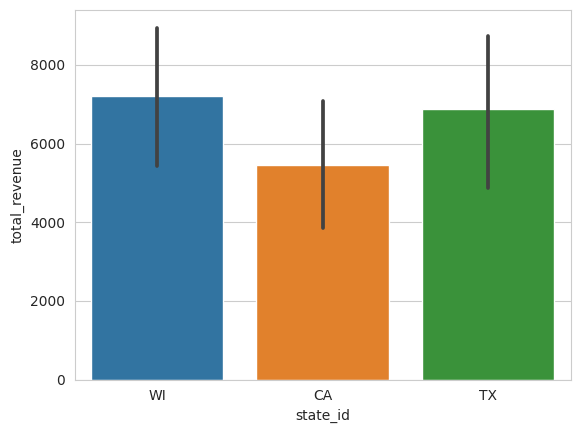
\includegraphics[scale=0.5]{41.png}

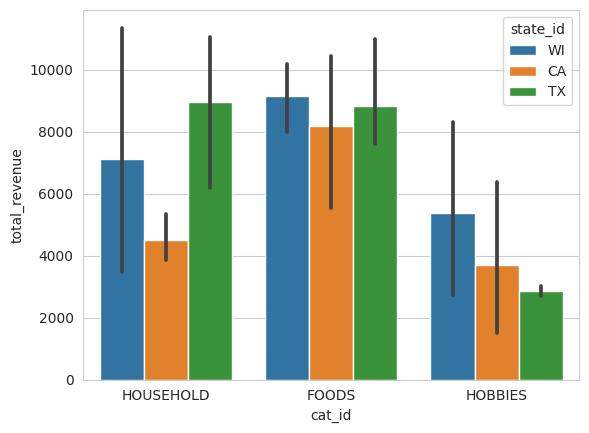
\includegraphics[scale=0.5]{42.png}


\item The next sections will be completed as we progress in our project.
\bigskip
\bigskip
%----------------------------------------------------------------------------------------
 % Algorithm and Methodology
%----------------------------------------------------------------------------------------


\section{Algorithm and Methodology}
We have implemented the following algorithms: 
\item \textbf {1. ARIMA (AutoRegressive Integrated Moving Average)}
\item A time series model that forecasts future values using past values and trends.
It consists of three elements: autoregression (AR), differencing (I), and moving average (MA).
Can be used to detect seasonality and trends in data, but only with stationary data.
Following hyperparameter tuning, our optimal p,q,d values are 1,1,1.
\item \textbf {2. SARIMAX((Seasonal AutoRegressive Integrated Moving Average with eXogenous factors)}
\item An ARIMA extension that accounts for seasonal patterns and allows for the inclusion of exogenous variables.
This model can handle both short-term and long-term seasonal patterns and includes seasonal P,D,Q values.
Can be used to assess the impact of external factors such as promotions or holidays on sales.
After hyperparameter tuning, our optimal values are (1,0,1),(0,1,1,7).
\item \textbf {3. PROPHET }
\item A simple time series model developed by Facebook that employs a decomposable additive model.
Can handle trend changes, seasonality, and holiday effects.
Allows for the inclusion of exogenous variables and includes a built-in mechanism for dealing with missing data and outliers.
To run the model, the ds(date) and y(attribute to be forecasted) columns are required.
\item \textbf {4. XGBOOST }
\item An ensemble of decision trees is used to predict in a machine learning model.
It is capable of handling non-linear relationships between predictors and targets.
Can automatically handle missing values and outliers.
Can be used to assess the impact of a variety of sales predictors, including promotions, weather, and economic indicators.
\item \textbf {5. LIGHTGBM }
\item LightGBM is a fast and high performing gradient boosting framework based on decision trees which grows leaf-wise and reduces memory usage with better accuracy. We have performed hyperparameter tuning using Optuna to get the best parameters and trained the LGBM Regressor model using these parameters which resulted in better performance of the model.

\item\textbf{Methodology}
Our team began by performing data preprocessing and exploratory data analysis (EDA) to gain insights into the Walmart sales dataset. We then implemented various time series models, including ARIMA, SARIMAX, and LightGBM, and utilized hyperparameter tuning to optimize the models' performance. We also combined multiple datasets, such as calendar, sell prices, and sales\_train\_validation, to enhance our analysis. With a training dataset spanning from 2011 to 2016 for all 30490 products, we predicted the sales for the next 28 days using the implemented algorithms. Finally, we compared the predicted results using sales\_train\_evaluation to obtain the RMSE values for all models. Our approach involved a combination of data science techniques and domain expertise to effectively forecast Walmart sales and identify key trends and factors driving product demand.
\bigskip
\bigskip
%----------------------------------------------------------------------------------------
 % Experiments and Results
%----------------------------------------------------------------------------------------
\section{Experiments and Results}
We have implemented 5 models. Out of all the algorithms implemented LightGBM performed better while XGBoost is the worst performing algorithm to forecast the sales. The table below lists the root mean squared error obtained for different models.

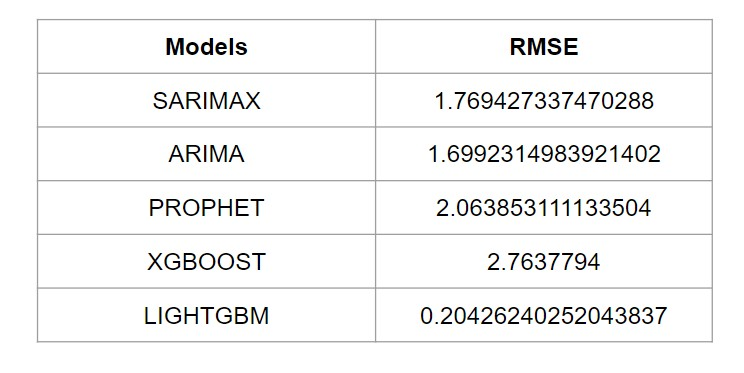
\includegraphics[scale=0.6]{models.jpg}
\item We have developed an application to forecast sales using the Flask framework and HTML. Below are the results for 2 different inputs as follows-
\\ \textbf{Scenario 1} :
If we want to see the sales of all categories(FOODS, HOUSEHOLD, HOBBIES) in all stores located in Texas, we will give input as TEXAS for the state field and 'ALL' for the remaining fields.

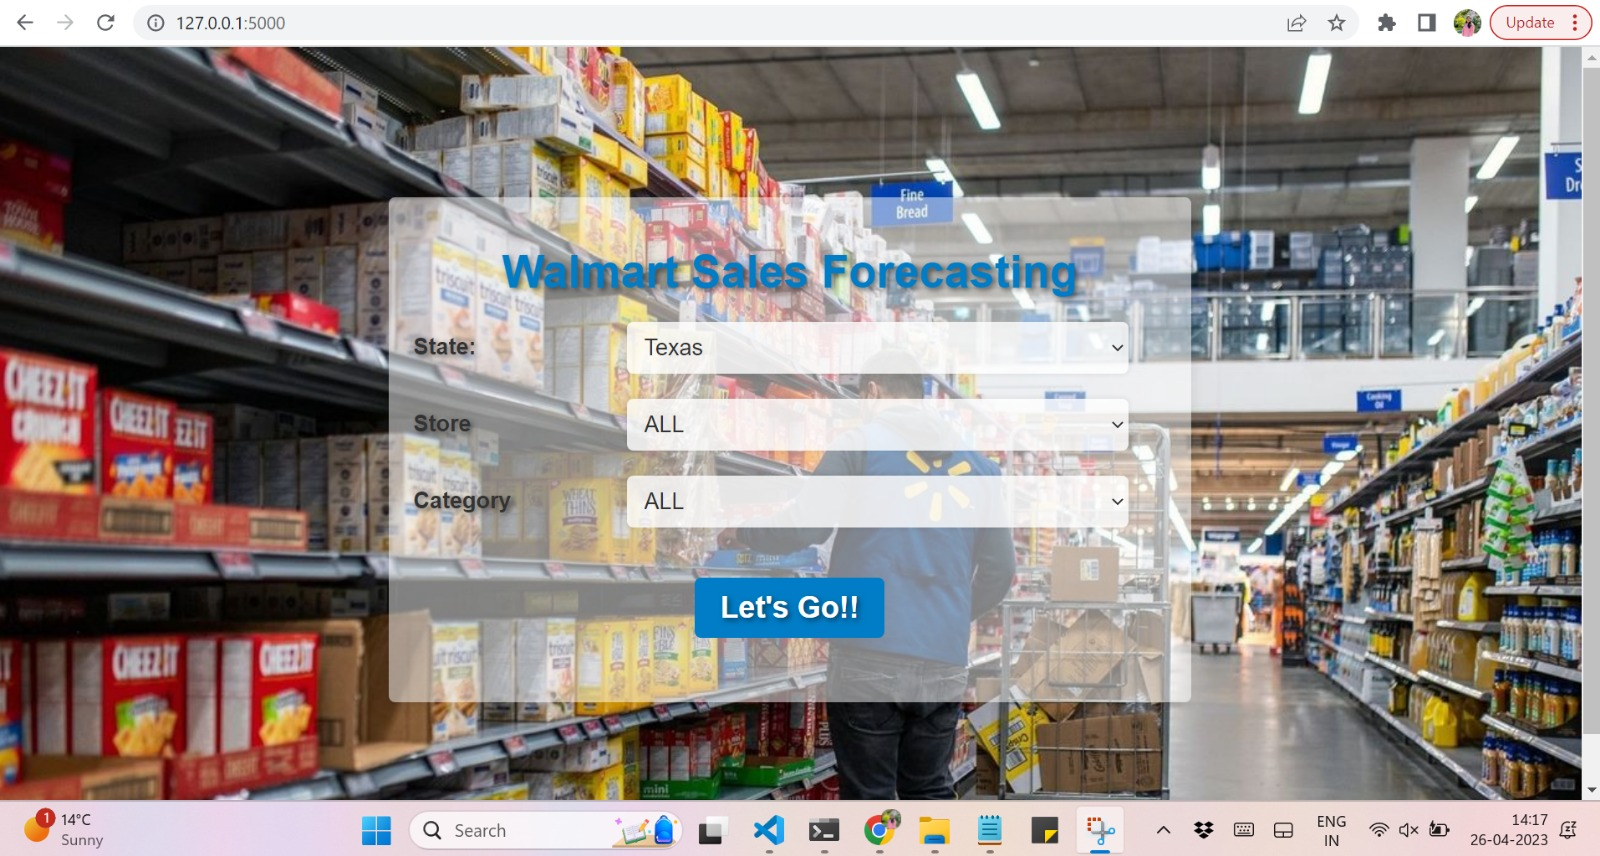
\includegraphics[scale=0.1]{1.jpeg}
\\Results obtained for the above input that shows sales of all categories in TX\_1, TX\_2 and TX\_3.

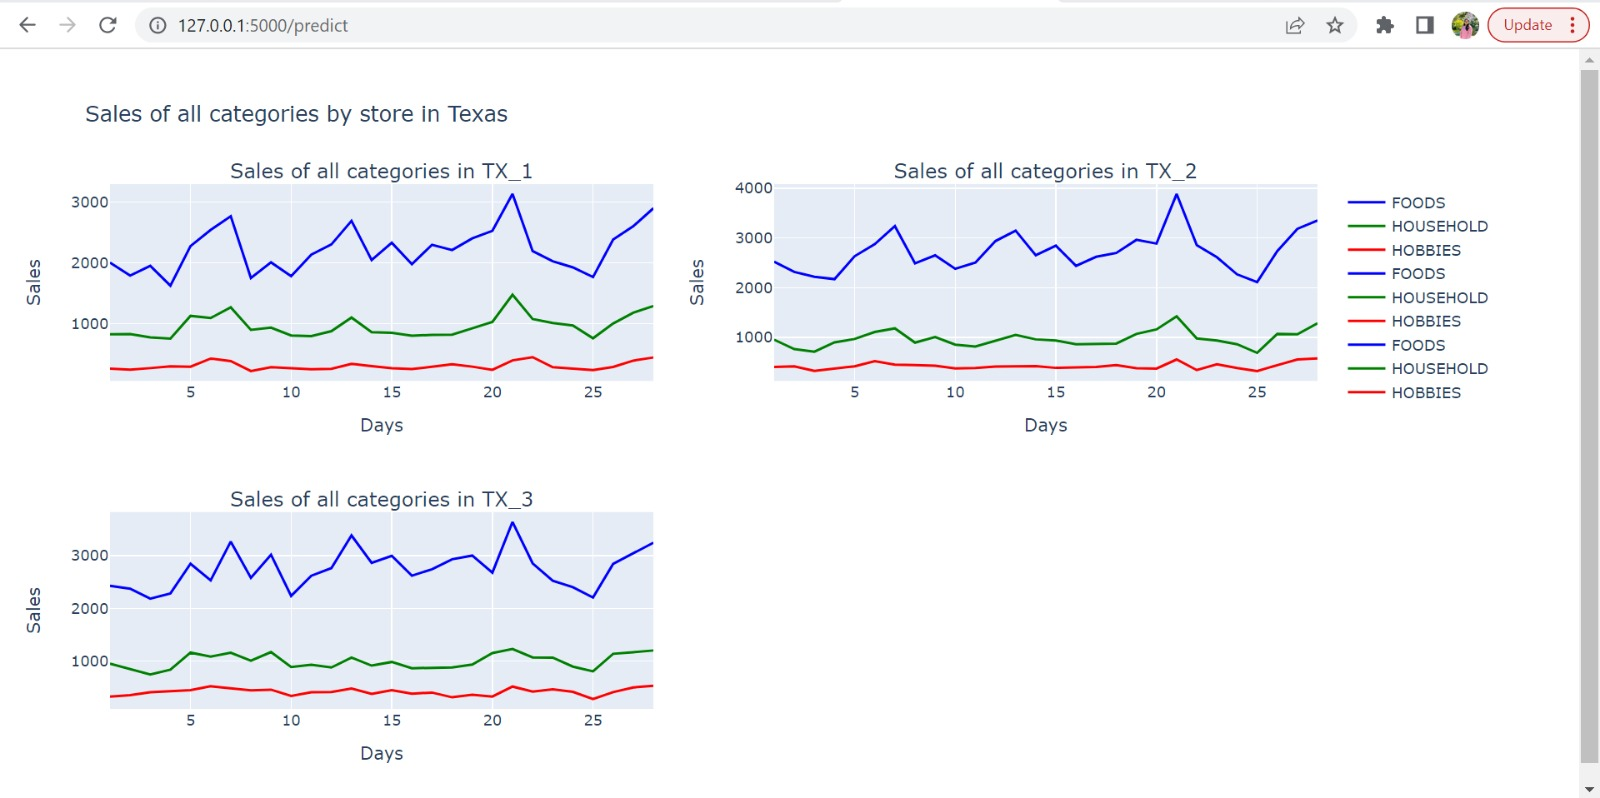
\includegraphics[scale=0.1]{2.jpeg}
\item\textbf{Scenario 2} :
Forecasting sales in a particular state in a particular category.

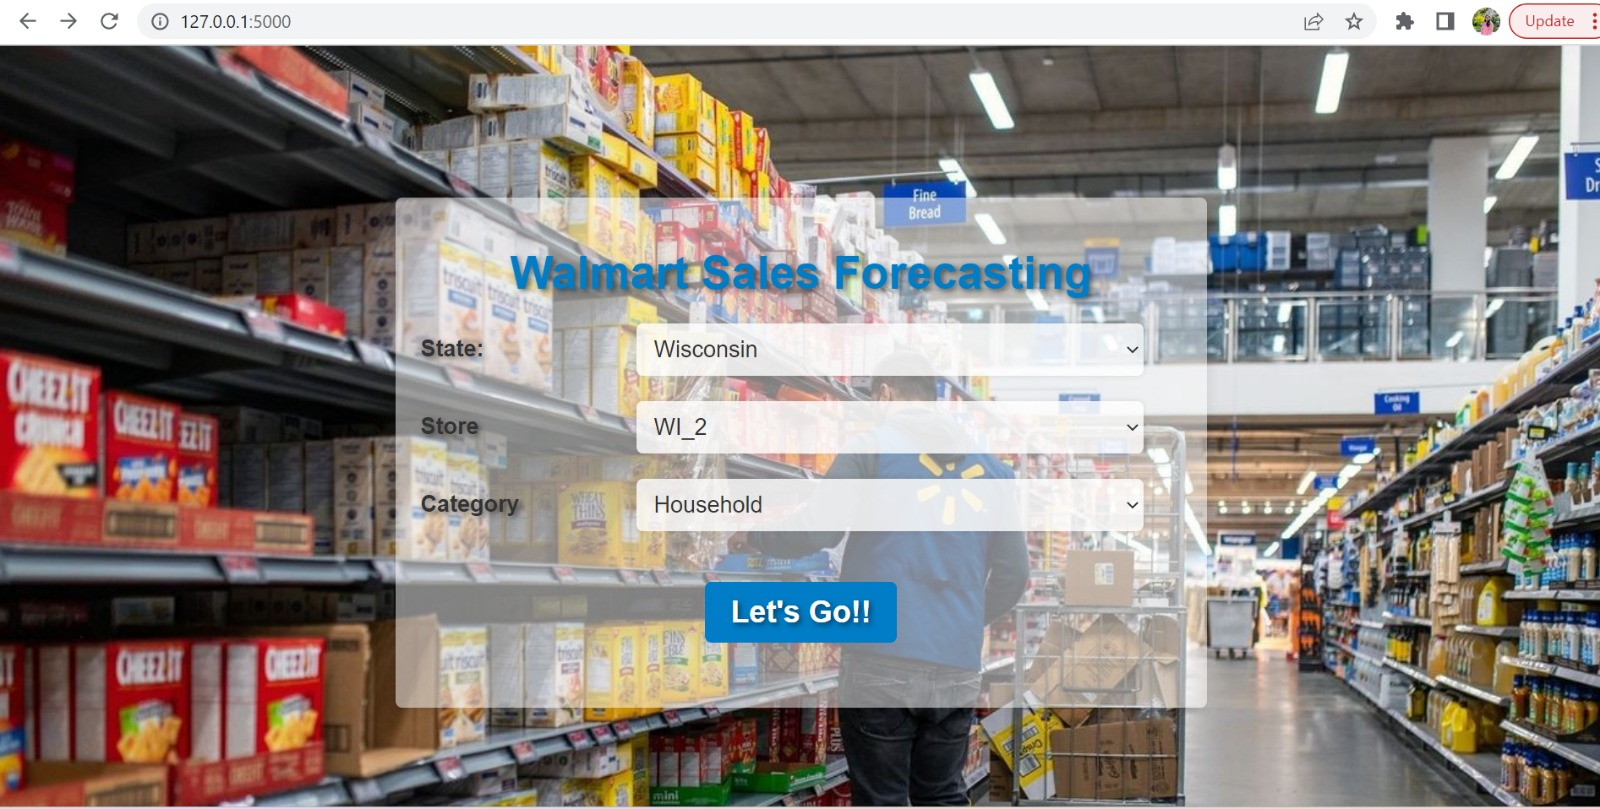
\includegraphics[scale=0.1]{3.jpeg}
\\ Results obtained for the above input that shows sales of HOUSEHOLD products in WI\_2

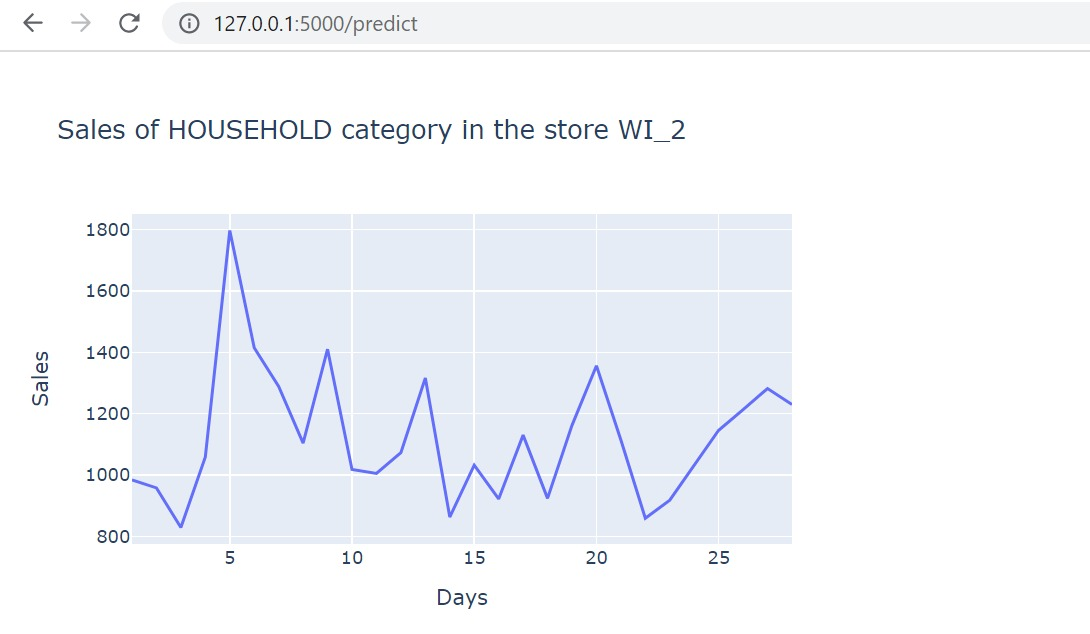
\includegraphics[scale=0.2]{4.jpeg}



\bigskip
\bigskip

%----------------------------------------------------------------------------------------
 %Deployement
%----------------------------------------------------------------------------------------
\section{Deployment and Maintenance}
Along with the M5 forecasting project, we also created a website using Flask and HTML to share our work with a larger audience. Users can easily interact with our models and browse the Walmart sales dataset on the website.


\item As part of our long-term strategy, we want to move the website and our models to a cloud platform for simpler access and maintenance. This guarantees that users can still access the website and that the models are continually updated with the most recent information. In order to enhance our models and give users better insights, we also plan to incorporate user feedback into the website.

\bigskip
\bigskip

%----------------------------------------------------------------------------------------
 % Summary and Conclusions
%----------------------------------------------------------------------------------------
\section{Summary and Conclusions}

The M5 forecasting project was a difficult but rewarding experience in which we attempted to forecast future sales of 30490 products across diverse stores. We have used five different forecasting algorithms, ARIMA, SARIMAX, PROPHET, XGBOOST, and LIGHTGBM, to accomplish this.

\\\item \\We have gained a thorough understanding of the challenges and complexities involved in using big data in the retail industry by working with vast amounts of data from Walmart. By examining such sizable datasets, we have gained valuable knowledge about customer behavior, inventory management, and sales forecasting. Because of this experience, we have also gotten better at data wrangling, exploratory data analysis, and machine learning, all of which are crucial for success in the field of data science. Because of this project, we have the skills and knowledge necessary for success in the data science sector, as well as a solid foundation for working with large, complex datasets.


\item \\In conclusion, using a variety of algorithms and evaluating their effectiveness has allowed us to better understand the data and determine the most effective forecasting strategy.  The accuracy and effectiveness of the models have increased because of the use of sophisticated techniques like hyperparameter tuning, which has given rise to invaluable insights into the potential future sales of the retail goods.

\phantomsection
\section*{Acknowledgments} % The \section*{} command stops section numbering
We owe a huge debt of gratitude to Indiana University Bloomington, our professor, and the Teaching Assistants for the priceless knowledge and abilities they have shared with us throughout this data mining course. Their commitment and diligence allowed us to complete the Walmart Sales forecasting project successfully and gain useful experience. We are now proficient with data mining tasks and have a solid understanding of all machine learning models. Utilizing superior data sets for assignments and projects has improved our knowledge. We will always be grateful for the advice, support, and lessons they have given us. From the bottom of our hearts, thank you!


\addcontentsline{toc}{section}{Acknowledgments} % Adds this section to the table of contents



%----------------------------------------------------------------------------------------
%	REFERENCE LIST
%----------------------------------------------------------------------------------------
\phantomsection
\bibliographystyle{unsrt}
\bibliography{sample}

\item \textbf{References}
\begin{enumerate}
    \item \href{https://www.kaggle.com/competitions/m5-forecasting-accuracy/overview}{https://www.kaggle.com/competitions/m5-forecasting-accuracy
    /overview}
\item\href{https://www.sciencedirect.com/science/article/pii/S0169207021001874}{https://www.sciencedirect.com/science/article
/pii/S0169207021001874}
\item \href{https://towardsdatascience.com/m5-forecasting-accuracy-24d7f42130de}{https://towardsdatascience.com/m5-forecasting-accuracy-24d7f42130de}

\end{enumerate}




%----------------------------------------------------------------------------------------

\end{document}